\section{eo\-Timed\-Monitor Class Reference}
\label{classeo_timed_monitor}\index{eoTimedMonitor@{eoTimedMonitor}}
Holds a collection of monitors and only fires them when a time limit has been reached.  


{\tt \#include $<$eo\-Timed\-Monitor.h$>$}

Inheritance diagram for eo\-Timed\-Monitor::\begin{figure}[H]
\begin{center}
\leavevmode
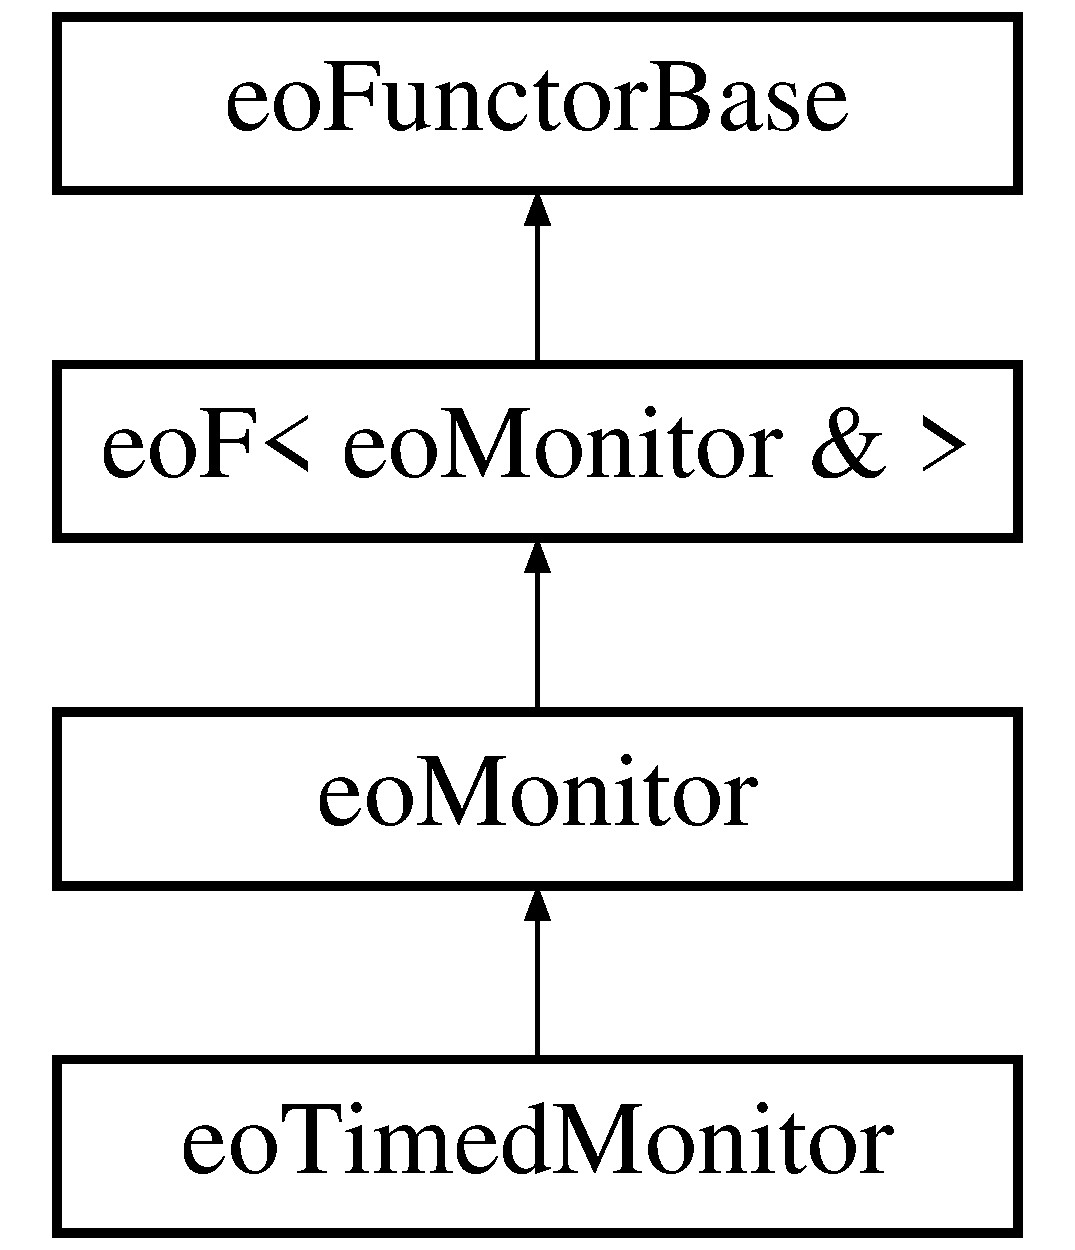
\includegraphics[height=4cm]{classeo_timed_monitor}
\end{center}
\end{figure}
\subsection*{Public Member Functions}
\begin{CompactItemize}
\item 
{\bf eo\-Timed\-Monitor} (int seconds\_\-)\label{classeo_timed_monitor_a0}

\item 
{\bf eo\-Monitor} \& {\bf operator()} (void)\label{classeo_timed_monitor_a1}

\begin{CompactList}\small\item\em The pure virtual function that needs to be implemented by the subclass. \item\end{CompactList}\item 
void {\bf add} ({\bf eo\-Monitor} \&mon)\label{classeo_timed_monitor_a2}

\item 
virtual std::string {\bf class\-Name} (void) const \label{classeo_timed_monitor_a3}

\end{CompactItemize}
\subsection*{Private Attributes}
\begin{CompactItemize}
\item 
clock\_\-t {\bf last\_\-tick}\label{classeo_timed_monitor_r0}

\item 
int {\bf seconds}\label{classeo_timed_monitor_r1}

\item 
std::vector$<$ {\bf eo\-Monitor} $\ast$ $>$ {\bf monitors}\label{classeo_timed_monitor_r2}

\end{CompactItemize}


\subsection{Detailed Description}
Holds a collection of monitors and only fires them when a time limit has been reached. 



Definition at line 40 of file eo\-Timed\-Monitor.h.

The documentation for this class was generated from the following file:\begin{CompactItemize}
\item 
eo\-Timed\-Monitor.h\end{CompactItemize}
